\section{Discussion}\label{section:discussion}

In this section we discuss the significance of the results presented in section \ref{section:results}.

\subsection{Single Language Clustering Setting}
The baseline NewsStand clustering method involves using machine translation and then constructing a TF-IDF vector and maintaining a time centroid for each cluster.
We found that this method generally led to better cluster assignments than using the LLMs we tested to generate cluster assignments.
In one case, using GPT-4o with the detailed system prompt, the NMI was higher than the baseline.
Surprisingly, adding article title, geo-coordinates, or timestamp information made the cluster assignments worse, even though that information is intuitively useful for determining which cluster an article belongs to.
This finding suggests that it is difficult (under our zero-shot setting) to get current LLMs to leverage multiple pieces of disparate intimation (timestamp, article text, coordinates) to decide an appropriate cluster for the articles.
Given the clear room for improvement, we suggest further work on using LLMs to cluster text with an emphasis on incorporating metadata like time and location associated with the text.
Few shot prompting is the logical next step to better leverage LLMs in this capacity.

\subsection{Cross-Lingual Clustering Setting}

Comparing the cross-lingual cluster assignments by time of publication, we found that the baseline method better accounted for time, with half of the clusters containing only articles that were published very close together in time (as opposed to none with GPT-4o).
Instead, GPT-4o grouped many articles together despite being published months apart, with the cluster assignment more correlated to language than time of publication.
Based on these results, it seems the baseline method that explicitly accounts for time of publication may be preferred for cross-lingual clustering where the time component is relevant, such as or news publications.

Based on our qualitative analysis of the cluster assignments produced by the LLMs, we found that the LLMs tended to group articles based on the language of the text, rather than the content or news story being described by the article.
This behavior was also consistent across our tests that added geo-coordinates or timestamps associated with the articles, for additional language independent context. 
Overall, we found that besides occasionally producing degenerate cluster assignments, LLMs tended not to leverage the article metadata, which is an area for future improvement that could lead to better clustering results.



% \subsection{Cross-Lingual Keyphrase Extraction}
% \nrscomment{discuss significance of LLM extracting proper nouns and corroborating findings of original paper or extracting something else, and why}

% \subsection{Cross-Lingual Cluster Correction}
% \nrscomment{discuss significance of improvement gained through cluster correction, by language.}

\begin{figure}[ht]
    \centering
    \begin{subfigure}[Timeline plot of the GPT-4o cluster assignments. 6 data points omitted to better see detail in different times.]{
        \centering
        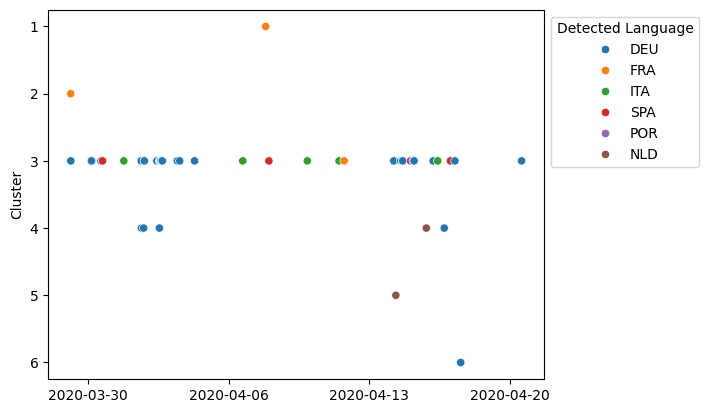
\includegraphics[width=0.5\textwidth]{data/images/timeline_plot_gpt4o.png}
        \label{fig:plot_gpt4o_time}
    }
    \end{subfigure}
    \vfill
    \begin{subfigure}[Timeline plot of the NewsStand cluster assignments. 6 data points omitted to better see detail in different times.]{
        \centering
        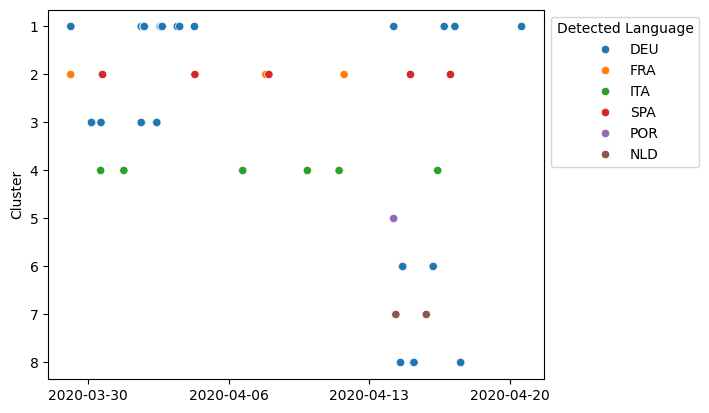
\includegraphics[width=0.5\textwidth]{data/images/timeline_plot_newsstand.png}
        \label{fig:plot_newsstand_time}
    }
    \end{subfigure}
    \caption{\textbf{Timeline plot of GPT-4o clusters vs baseline NewsStand clusters.}}\label{figure:time-plots} 
\end{figure}